%-----------------------------------------------------------------------------%
\chapter{\babTiga}
%-----------------------------------------------------------------------------%
Bagian ini menjelaskan metodologi penelitian termasuk di dalamnya pendekatan penelitian dan tahapan penelitian yang digunakan penulis dalam melakukan penelitian.
%-----------------------------------------------------------------------------%
\section{Pendekatan Penelitian}
%-----------------------------------------------------------------------------%

Penelitian ini  menggunakan pendekatan studi kasus. Cresswell (\citeyear{papper.Creswell}), pendekatan studi kasus adalah penelitian tentang suatu program, peristiwa, aktivitas, proses, atau kelompok individu.
\linebreak\linebreak
Pendekatan studi kasus yang dilakukan adalah proses pembelajaran mahasiswa Fakultas Ilmu Komputer di Universitas Indonesia pada mata kuliah Dasar Dasar Pemrograman. Penelitian ini berusaha memahami perasaan responden terhadap suatu masalah. Penelitian ini dilakukan tanpa faktor - faktor eksternal sehingga tidak mempengaruhi pemikiran responden.
\linebreak\linebreak
Penelitian yang dilakukan menggunakan pendekatan \textit{Mixed method} sebagai \textit{research design}. \textit{Mixed method} merupakan metode yang menggabungkan pendekatan kuantitatif dan kualitatif (Creswell, 2013). Pendekatan yang bersifat kualitatif dilakukan dengan cara menyusun kuesioner yang mencampur pertanyaan \textit{close-ended} dan \textit{open-ended} dengan tujuan untuk mendapatkan requirement yang paling sesuai untuk diterapkan pada situs pembelajaran yang akan dikembangkan. Pendekatan yang bersifat kuantitatif dilakukan dalam pengolahan data dengan tujuan untuk membantu pengambilan keputusan.
\linebreak\linebreak
Dalam pengembangan sistem ini penulis menggunakan pendekatan model ADDIE  (Morisson et al., \citeyear{book.morisson}). Secara singkat model pengembangan ADDIE merupakan kepanjangan dari \textit{Analyze, Design, Develop, Implement, and Evaluate.}

%-----------------------------------------------------------------------------%
\section{Tahapan Penelitian}
%-----------------------------------------------------------------------------%

Dalam penelitian ini penulis melakukan beberapa tahapan sesuai dengan Gambar 3.1.

\begin{figure}
	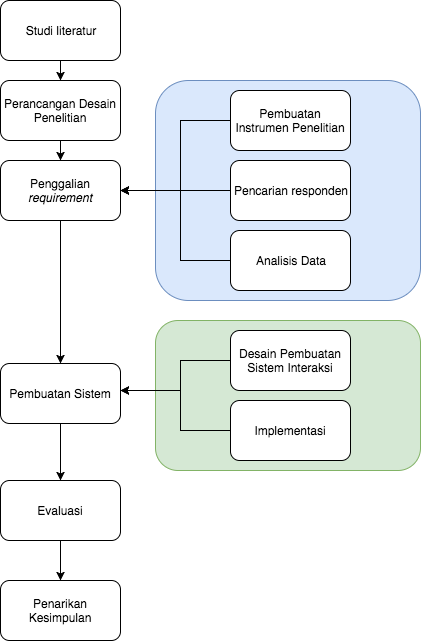
\includegraphics[scale=0.9]{pics/flow-pembuatan}
	\caption{Alur tahapan penelitian}
	\centering
\end{figure}
\

	%-----------------------------------------------------------------------------%
	\subsection{Studi literatur}
	%-----------------------------------------------------------------------------%
	
	Untuk memulai penelitian, penulis terlebih dahulu melakukan studi literatur dengan
	mengacu kepada konsep \textit{Game} and \textit{Learning} yang
	diperkenalkan oleh Kirriemuir (2004) dan membaca penelitian serupa yang sebelumnya telah dilakukan. Penulis juga mengumpulkan sumber-sumber pendukung latar belakang dan tujuan penelitian menggunakan online library, seperti IEEE Xplore, Google Scholar. Selain itu penulis juga menggunakan buku - buku yang dipinjam dari lab Digital Library and Distance Learning.
	
	%-----------------------------------------------------------------------------%
	\subsection{Instrumen penelitian}
	%-----------------------------------------------------------------------------%
	
	Dalam pelaksanaan penelitian ini, beberapa instrumen penelitian yang perlu dipersiapkan, antara lain:
	
	\begin{enumerate}
		\item Kuesioner \textit{online} yang memuat waktu, kesulitan, cara, dan tingkat pemahaman responden dalam memahami materi dasar dasar pemrograman.
		\item Daftar pertanyaan wawancara untuk mengetahui pendapat yang telah menajalani pembelajaran pada mata kuliah dasar dasar pemrograman.
	\end{enumerate}

	Dari instrumen penelitian ini dipersiapkan pada tahap awal perencanaan evaluasi. Instrumen ini dibutuhkan untuk menggali \textit{requirement} dalam membangun sistem interaksi pembelajaran berbasis permainan.
	
	%-----------------------------------------------------------------------------%
	\subsection{Analisis dan Representasi Data}
	%-----------------------------------------------------------------------------%
	
	Dalam penelitian ini, penulis melakukan teknik data analisis \textit{simple qualitative analysis} dengan mengkategorisasikan data. Data yang berupa pilihan langsung oleh responden akan dihitung frequensi pemilihnya. Data yang berupa isian akan dikelompokkan berdasarkan unik respon dari responden dengan. Pengelompokan data dalam bentuk kodifikasi.
	\begin{table}
		\centering
		\caption{Kodifikasi pertanyaan \textit{open-ended}}
		\label{tab:tab1}
		\begin{tabular}{| c | c |}
			\hline
			Kode & Pertanyaan \\
			\hline
			PP[N] & \multicolumn{1}{p{10cm}|}{Menurut anda apakah itu pemrograman?}\\ \hline
			JG[N] & \multicolumn{1}{p{10cm}|}{Menurut anda, jenis \textit{game} seperti apa yang dapat membantu anda dalam mengimplementasikan dan memahami materi pembelajaran pemrograman??} \\ \hline
		\end{tabular}
		\vspace{1ex}
		
		\raggedright \small{N = angka yang menampilkan jenis jawaban ke-n}
	\end{table}
	Hasil dari analisis evaluasi kemudian dilanjutkan ketahap implementasi sistem. Dalam tahapan ini, digunakan \textit{Eight Golden Rules of User Interface Design} yang dirumuskan oleh Shneiderman dan Plaisant (\citeyear{papper.shneiderman}) dan digunakan dasar teori pengembangan \textit{Game Base Learning} oleh Kirriemuir (2004).
	
	%-----------------------------------------------------------------------------%
	\subsection{Pengujian Prototipe Sistem dengan \textit{Usability Testing}}
	%-----------------------------------------------------------------------------%
	
	Setelah tahap pembuatan prototipe selesai, penulis melakukan uji sistem dengan menggunakan \textit{usability testing} dan disertai kuisoner untuk saran dan kritik terhadap sistem yang telah penulis rangkai. Dari hasil pengujian, penulis menggunakan data tersebut untuk melakukan proses penarikan kesimpulan. Skenario untuk pengujian UT terdapat pada Lampiran 2 dan Hasil responden akan ditampilkan pada Lampiran 3
	
	%-----------------------------------------------------------------------------%
	\subsection{Pengambilan Kesimpulan Penelitian}
	%-----------------------------------------------------------------------------%
	
	Setelah melalui tahap \textit{usability testing}, penulis melakukan penarikan kesimpulan yang menghasilkan jawaban yang menjawab rumusan masalah yang dijabarkan pada bab satu. Tahapan ini akan dijelaskan pada bab keempat, dan kesimpulan akan dijabarkan pada bab kelima, bersama dengan saran untuk penelitian yang akan dilakukan di masa mendatang.
	

